\iffalse
\author{EE24BTECH11047}
\section{ph}
\chapter{2012}
\fi
	\item The polarizability of the hydrogen atom in unit of $\brak{C^2m/N}$ is
    \begin{enumerate}
        \item $2.0 \times 10^{-40}$
        \item $1.4 \times 10^{-41}$
        \item $1.4 \times 10^{-40}$
        \item $2.0 \times 10^{-39}$
    \end{enumerate}

\textbf{Statement for Linked Answer Questions 54 and 55:}\\ 
 A particle of mass $m$ slides under the gravity without friction along the parabolic path $y = ax^2$ as shown in the figure. Here $a$ is a constant.\\
     \begin{figure}[!ht]
    \centering
    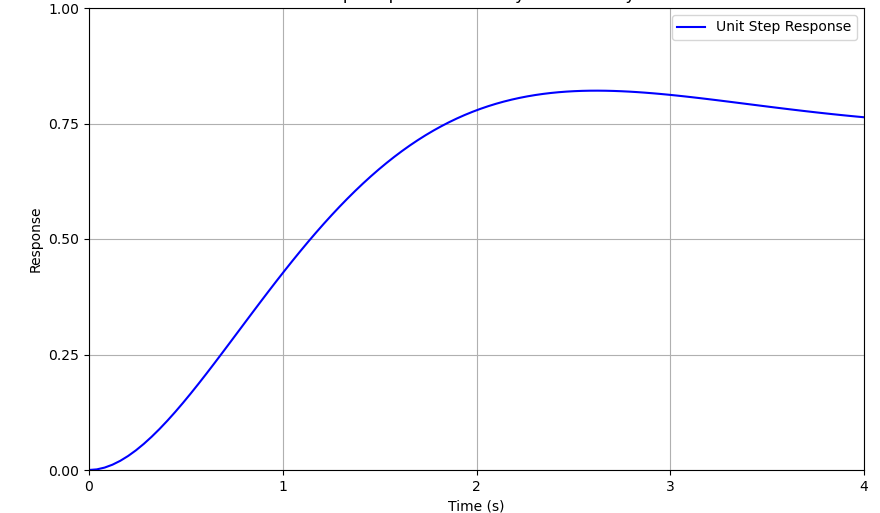
\includegraphics[width=2.5cm]{./GATE-yearwise/2009/figs/fig1.png}
    \end{figure}
\item The Lagrangian for this particle is given by,
    \begin{enumerate}
        \item $L = \frac{1}{2} m\dot{x}^2 - mgax^2$
	\item $L = \frac{1}{2} m\brak{1 + 4a^2x^2}\dot{x}^2 - mgax^2$
        \item $L = \frac{1}{2} m\dot{x}^2 + mgax^2$
	\item $L = \frac{1}{2} m\brak{1 + 4a^2x^2}\dot{x}^2 + mgax^2$
    \end{enumerate}

\item The Lagrange's equation of motion of the particle is
    \begin{enumerate}
        \item $\ddot{x} = 2gax$
	\item $m\brak{1 + 4a^2x^2}\ddot{x} = -2mgax - 4ma^2x\dot{x}^2$
	\item $m\brak{1 + 4a^2x^2}\ddot{x} = 2mgax + 4ma^2x\dot{x}^2$
        \item $\ddot{x} = -2gax$
    \end{enumerate}

\item Choose the grammatically \textbf{INCORRECT} sentence:
    \begin{enumerate}
        \item They gave us the money back less the service charges of Three Hundred rupees.
        \item This country's expenditure is not less than that of Bangladesh.
        \item The committee initially asked for a funding of Fifty Lakh rupees, but later settled for a lesser sum.
        \item This country's expenditure on educational reforms is very less.
    \end{enumerate}

\item Which one of the following options is the closest in meaning to the word given below?\\
\textbf{Mitigate}
    \begin{enumerate}
        \item Diminish
        \item Divulge
        \item Dedicate
        \item Denote
    \end{enumerate}

\item Choose the most appropriate alternative from the options given below to complete the following sentence:  
\textbf{Despite several \underline{\hspace{1cm}} the mission succeeded in its attempt to resolve the conflict.}
    \begin{enumerate}
        \item attempts
        \item setbacks
        \item meetings
        \item delegations
    \end{enumerate}

\item The cost function for a product in a firm is given by $5q^2$, where $q$ is the amount of production. The firm can sell the product at a market price of $Rs. 50$ per unit. The number of units to be produced by the firm such that the profit is maximized is:
    \begin{enumerate}
        \item 5
        \item 10
        \item 15
        \item 25
    \end{enumerate}

\item Choose the most appropriate alternative from the options given below to complete the following sentence:  
	\textbf{Suresh's dog is the one \underline{\hspace{1cm}} was hurt in the stampede.}
    \begin{enumerate}
        \item that
        \item which
        \item who
        \item whom
    \end{enumerate}

\item Which of the following assertions are CORRECT?\\
        P: Adding 7 to each entry in a list adds 7 to the mean of the list.\\
        Q: Adding 7 to each entry in a list adds 7 to the standard deviation of the list.\\
        R: Doubling each entry in a list doubles the mean of the list.\\
        S: Doubling each entry in a list leaves the standard deviation of the list unchanged.
    \begin{enumerate}
        \item P, Q
        \item Q, R
        \item P, R
        \item R, S
    \end{enumerate}

\item An automobile plant contracted to buy shock absorbers from two suppliers X and Y. X supplies $60\%$ and Y supplies $40\%$ of the shock absorbers. All shock absorbers are subjected to a quality test. The ones that pass the quality test are considered reliable. Of X's shock absorbers, $96\%$ are reliable. Of Y's shock absorbers, $72\%$ are reliable.  
The probability that a randomly chosen shock absorber, which is found to be reliable, is made by Y is:
    \begin{enumerate}
        \item 0.288
        \item 0.334
        \item 0.667
        \item 0.720
    \end{enumerate}

\item A political party ordes an arch for the entrance to the ground in which the annual convention is being held. The profile of the arch follows the equation $y = 2x - 0.1x^2$ where $y$ is the height of the arch in meters. The maximum possible height of the arch is:
    \begin{enumerate}
        \item 8 meters
        \item 10 meters
        \item 12 meters
        \item 14 meters
    \end{enumerate}

\item Wanted Temporary, part-time persons for the post of Field Interviewer to conduct personal interviews to collect and collate economic data. Requirements: High school pass, must be available for day, evening, and Saturday work. Transportation paid, expenses reimbursed.  
Which one of the following is the best inference from the above advertisement?
    \begin{enumerate}
        \item Gender-discriminatory
        \item Xenophobic
        \item Not designed to make the post attractive
        \item Not gender-discriminatory
    \end{enumerate}

\item Given the sequence of terms: AD, CG, FK, JP, the next term is:
    \begin{enumerate}
        \item OV
        \item OW
        \item PV
        \item PW
    \end{enumerate}

r
